\section{User-based evaluation} % to refactor

\subsection{Methodology}

% Evaluation of three explanations: a structured one generated from a template, an LLM-generated explanation based on the graph structure, and an LLM-generated explanation based on the template.

Part of our project's goal was to perform a user-based evaluation of the three types of explanations generated by our pipeline. We drew inspiration from \cite{balog2020measuring} to craft the structure for our evaluation procedure (Fig.~\ref{fig:UserEvalStructure}), albeit with slight modifications due to the inclusion of LLM-generated explanations. We decided to focus on the following key aspects:
\begin{enumerate}
    \item Assessing user expectations of recommendation explanations using the seven goals from \cite{tintarev2015explaining}, also used by \cite{balog2020measuring}.
    \item Presenting a recommended item to the user alongside multiple alternative explanations (based on a watching profile selected by the user beforehand).
    \item Requesting users to assess the explanations based on their general preference and measure the extent to which each explanation satisfies the seven goals.
          %\item Collecting qualitative insights through open questions about user expectations toward recommendation explanations and assessments of the current ones.
    \item Gathering qualitative insights via open question on user expectations and explanation assessments.
\end{enumerate}

\begin{figure}[!ht]
    \centering
    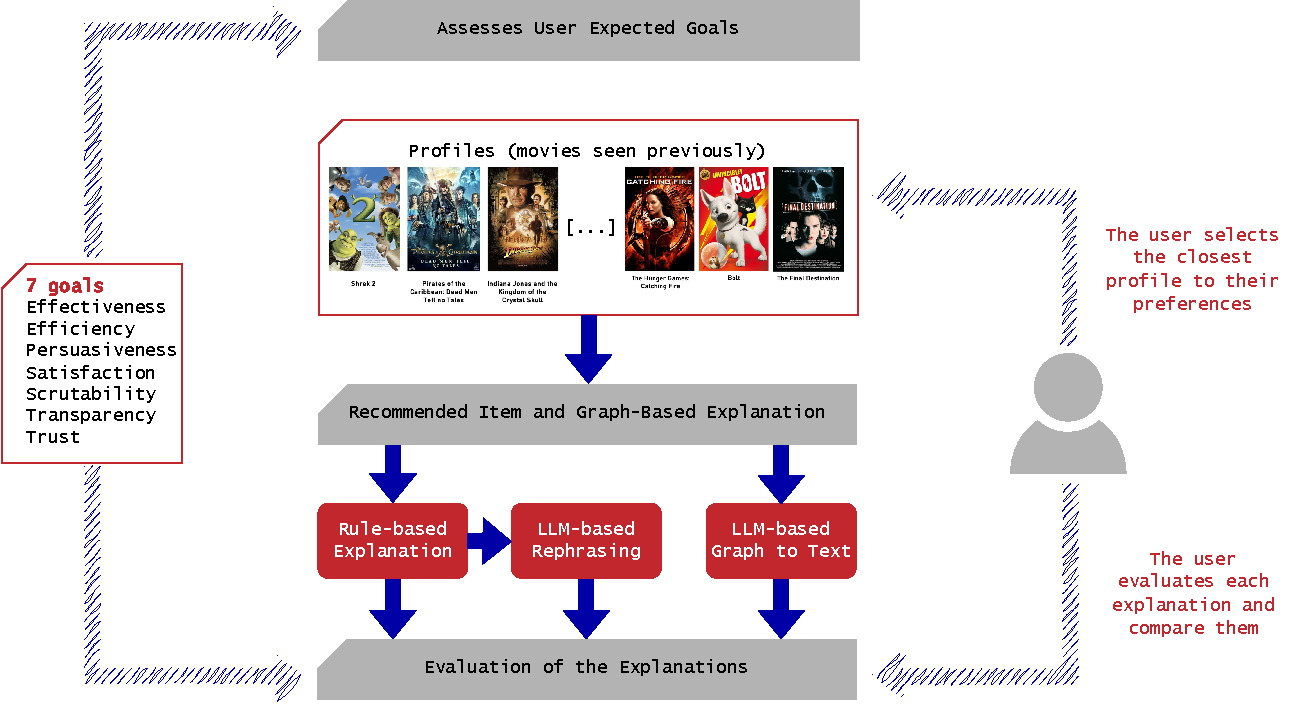
\includegraphics[width=\linewidth]{images/UserEval.pdf}
    \caption{Structure of our user evaluation procedure}
    \label{fig:UserEvalStructure}
\end{figure}

% With the evaluation structure in place, we implemented it using Microsoft Forms. We refined the question formulations to ensure clarity and relevance.
Afterward, we conducted a dry run to validate the clarity of the questionnaire and assess its length to prevent evaluator fatigue. Subsequently, we rolled out the questionnaire to multiple evaluators to gather their responses.

\subsection{Results}

We conducted 25 user tests with TRAIL'23 Workshop participants (researchers in AI). The small number of participants means that no statistically robust conclusions can be drawn, but certain trends can be observed.
% Concerning the user expectations about explanations (see Fig.~\ref{fig:ResultsExpectation}, we observe similar importance for the different goals investigated. 

% \begin{figure}[!ht]
%     \centering
%     \includesvg[width=\linewidth]{images/expectation_results.svg}
%     \caption{User expectation about the recommendation explanations w.r.t. the 7 goals.}
%     \label{fig:ResultsExpectation}
% \end{figure}

Concerning the user's expectations about explanations, we observe no difference in importance for the seven goals investigated. However, concerning user assessment of the generated explanations (see Fig.~\ref{fig:ResultsExplanation}), we observe that the explanation generated by the LLM from a knowledge graph performs best w.r.t. the 7 goals. And this result is confirmed by the participants' general assessment of the explanations. According to the participants, this explanation type is mainly preferred because it's often more detailed and more pleasant to read.
However, beyond the small sample size ($n = 25$), it is important to point out the significant variance in these last results. This indicates strong differences between participants in the way they perceive explanations, which is a result that should be investigated further.

\begin{figure}[!ht]
    \centering
    \includesvg[width=\linewidth]{images/explanation_results.svg}
    \caption{User assessment of explanations w.r.t. the 7 goals. about the recommendation explanations.}
    \label{fig:ResultsExplanation}
\end{figure}


Moreover, we observed that LLMs often introduce additional details. Although most of them seem correct, they do not come from the knowledge graph and are therefore not verified. This may be due to the model's ability to draw on cultural references~\cite{reynolds2021prompt}, in this case, movie titles. If this is undesirable, a workaround is to use numbered labels instead of movie titles. This will limit the model only to use in-context information.


% This prevents the model from accessing movie-specific knowledge, ensuring the generated content follows the provided knowledge graph or template. 

% We collected and analyzed the results, focusing on the following aspects:
% \begin{itemize}
%     \item Investigating differences between the importance of goals and their actual satisfaction.
%     \item Assessing whether the explanations fulfil users' expected goals.
%     \item Examining overall satisfaction differences among explanation types.
%     \item Exploring correlations between overall satisfaction and individual goals.
%     \item Investigating goal interdependencies and correlations.
% \end{itemize}